\documentclass[tikz,border=3.14mm]{standalone}
\usepackage{tikz}
\usetikzlibrary{positioning} % Útil para posicionamento relativo
\begin{document}

\begin{figure}[h!]
\centering
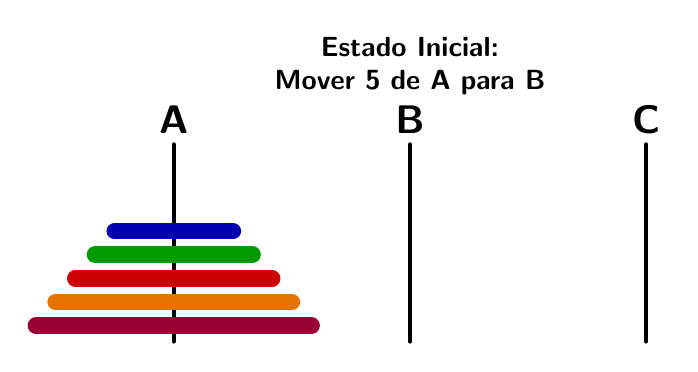
\begin{tikzpicture}[
    pin/.style={black, ultra thick, line cap=round},
    disk/.style={line width=6pt, line cap=round},
    disk1/.style={disk, blue!70!black}, disk2/.style={disk, green!60!black},
    disk3/.style={disk, red!80!black}, disk4/.style={disk, orange!90!black},
    disk5/.style={disk, purple!80!black},
    pin_label/.style={font=\Large\sffamily\bfseries},
    step_label/.style={align=center, font=\sffamily\bfseries, yshift=0.5cm}
]
    \node[step_label] at (3, 3) {Estado Inicial:\\Mover 5 de A para B};
    % Pinos
    \draw[pin] (0,0) -- ++(0,2.5) node[pin_label, above] {A};
    \draw[pin] (3,0) -- ++(0,2.5) node[pin_label, above] {B};
    \draw[pin] (6,0) -- ++(0,2.5) node[pin_label, above] {C};
    % Discos em A
    \draw[disk5] (-1.75, 0.2) -- (1.75, 0.2);
    \draw[disk4] (-1.5, 0.5) -- (1.5, 0.5);
    \draw[disk3] (-1.25, 0.8) -- (1.25, 0.8);
    \draw[disk2] (-1.0, 1.1) -- (1.0, 1.1);
    \draw[disk1] (-0.75, 1.4) -- (0.75, 1.4);
\end{tikzpicture}
\caption{Estado inicial com 5 discos no pino de origem A.}
\end{figure}

\begin{figure}[h!]
\centering
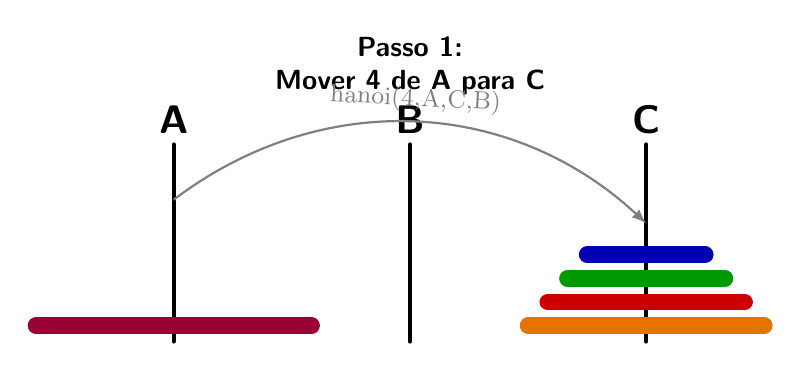
\begin{tikzpicture}[
    pin/.style={black, ultra thick, line cap=round},
    disk/.style={line width=6pt, line cap=round},
    disk1/.style={disk, blue!70!black}, disk2/.style={disk, green!60!black},
    disk3/.style={disk, red!80!black}, disk4/.style={disk, orange!90!black},
    disk5/.style={disk, purple!80!black},
    pin_label/.style={font=\Large\sffamily\bfseries},
    step_label/.style={align=center, font=\sffamily\bfseries, yshift=0.5cm},
    move_arrow/.style={-latex, thick, gray, bend left=40}
]
    \node[step_label] at (3, 3) {Passo 1:\\Mover 4 de A para C};
    % Pinos
    \draw[pin] (0,0) -- ++(0,2.5) node[pin_label, above] {A};
    \draw[pin] (3,0) -- ++(0,2.5) node[pin_label, above] {B};
    \draw[pin] (6,0) -- ++(0,2.5) node[pin_label, above] {C};
    % Discos
    \draw[disk5] (-1.75, 0.2) -- (1.75, 0.2); % Disco maior fica em A
    \draw[disk4] (4.5, 0.2) -- (7.5, 0.2);   % Pilha menor (n-1) vai para C
    \draw[disk3] (4.75, 0.5) -- (7.25, 0.5);
    \draw[disk2] (5.0, 0.8) -- (7.0, 0.8);
    \draw[disk1] (5.25, 1.1) -- (6.75, 1.1);
    % Seta do movimento recursivo
    \draw[move_arrow] (0,1.8) to node[above, midway, sloped] {\small hanoi(4,A,C,B)} (6,1.5);
\end{tikzpicture}
\caption{Resultado do primeiro passo recursivo: mover a pilha de 4 discos para o pino auxiliar.}
\end{figure}

\begin{figure}[h!]
\centering
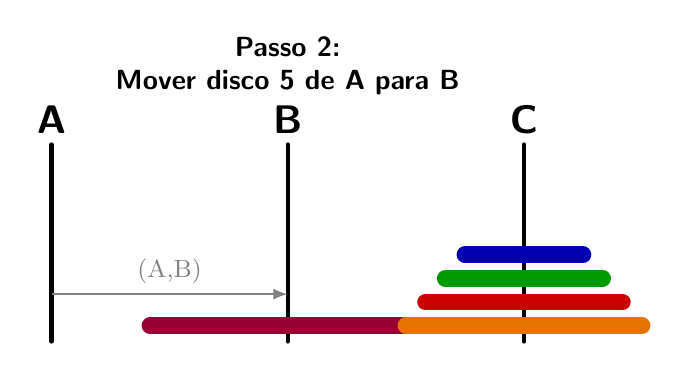
\begin{tikzpicture}[
    pin/.style={black, ultra thick, line cap=round},
    disk/.style={line width=6pt, line cap=round},
    disk1/.style={disk, blue!70!black}, disk2/.style={disk, green!60!black},
    disk3/.style={disk, red!80!black}, disk4/.style={disk, orange!90!black},
    disk5/.style={disk, purple!80!black},
    pin_label/.style={font=\Large\sffamily\bfseries},
    step_label/.style={align=center, font=\sffamily\bfseries, yshift=0.5cm},
    move_arrow/.style={-latex, thick, gray, bend left=40}
]
    \node[step_label] at (3, 3) {Passo 2:\\Mover disco 5 de A para B};
    % Pinos
    \draw[pin] (0,0) -- ++(0,2.5) node[pin_label, above] {A};
    \draw[pin] (3,0) -- ++(0,2.5) node[pin_label, above] {B};
    \draw[pin] (6,0) -- ++(0,2.5) node[pin_label, above] {C};
    % Discos
    \draw[disk5] (1.25, 0.2) -- (4.75, 0.2); % Disco maior movido para B
    \draw[disk4] (4.5, 0.2) -- (7.5, 0.2);
    \draw[disk3] (4.75, 0.5) -- (7.25, 0.5);
    \draw[disk2] (5.0, 0.8) -- (7.0, 0.8);
    \draw[disk1] (5.25, 1.1) -- (6.75, 1.1);
    % Seta do movimento
    \draw[move_arrow, bend left=0] (0,0.6) to node[above, midway] {\small (A,B)} (3,0.6);
\end{tikzpicture}
\caption{O movimento do disco base (o maior) da origem para o destino.}
\end{figure}

\begin{figure}[h!]
\centering
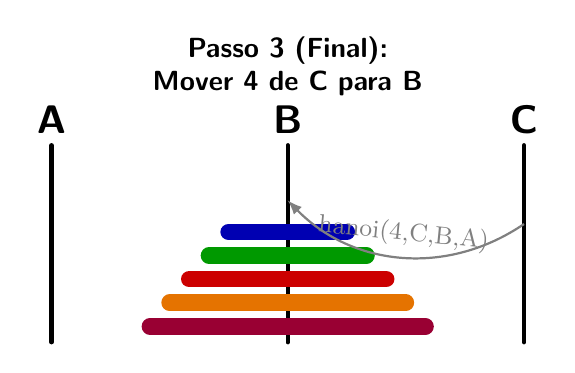
\begin{tikzpicture}[
    pin/.style={black, ultra thick, line cap=round},
    disk/.style={line width=6pt, line cap=round},
    disk1/.style={disk, blue!70!black}, disk2/.style={disk, green!60!black},
    disk3/.style={disk, red!80!black}, disk4/.style={disk, orange!90!black},
    disk5/.style={disk, purple!80!black},
    pin_label/.style={font=\Large\sffamily\bfseries},
    step_label/.style={align=center, font=\sffamily\bfseries, yshift=0.5cm},
    move_arrow/.style={-latex, thick, gray, bend left=40}
]
    \node[step_label] at (3, 3) {Passo 3 (Final):\\Mover 4 de C para B};
    % Pinos
    \draw[pin] (0,0) -- ++(0,2.5) node[pin_label, above] {A};
    \draw[pin] (3,0) -- ++(0,2.5) node[pin_label, above] {B};
    \draw[pin] (6,0) -- ++(0,2.5) node[pin_label, above] {C};
    % Discos
    \draw[disk5] (1.25, 0.2) -- (4.75, 0.2); % Pilha final em B
    \draw[disk4] (1.5, 0.5) -- (4.5, 0.5);
    \draw[disk3] (1.75, 0.8) -- (4.25, 0.8);
    \draw[disk2] (2.0, 1.1) -- (4.0, 1.1);
    \draw[disk1] (2.25, 1.4) -- (3.75, 1.4);
    % Seta do movimento recursivo
    \draw[move_arrow] (6,1.5) to node[above, midway, sloped] {\small hanoi(4,C,B,A)} (3,1.8);
\end{tikzpicture}
\caption{Resultado do último passo recursivo: mover a pilha de 4 discos do auxiliar para o destino.}
\end{figure}

\end{document}
